\documentclass{IEEEtran}
\usepackage{amssymb, amsmath, amsthm}
\usepackage{verbatim}
\usepackage{graphicx}
\usepackage{hyperref} % \url \href

\newcommand{\pfrac}[2]{\frac{\partial #1}{\partial #2}}
\newcommand{\calx}{\mathcal{X}}
\newtheorem{definition}{Definition}
\newtheorem{proposition}{Proposition}
% \renewcommand{\H}{\mathcal{H}}
\usepackage[style=ieee, backend=bibtex, sorting=none]{biblatex}
\addbibresource{ReferenceForReview.bib}

\begin{document}

\title{Review of Rotational Equivariant Convolution Neural Networks}
%\author{
%    \IEEEauthorblockN{Wenhao Zhang} \\
%    \IEEEauthorblockA{National Institute of Materials Science, Tsukuba}    
%}
\author{Wenhao Zhang \\ National Institute of Materials Science, Tsukuba}
\date{\today}

\maketitle

\begin{abstract}
    Convolution neural network are very successful in that, through weight sharing convolution and pooling, higher and higher abstraction 
    of the original input are can be generated approximately equivariantly, i. e.\,, translation properties of the input (in most case image)
    are kept until at late stage. Weight sharing also greatly reduced the number of parameter, making it easier to be trained. 
    Recently, there are many attempts to generalize the standard convolution network and make them rotational equivariant so that the information
    about how an image is rotated is also kept throughout the network until late stage. This is a highly desirable property for machine learning 
    on materials structures. For example, if we want to predict the atomic force on the atom from its local environment. Such rotation equivariance 
    because necessary because we want the predicted force to rotate in the same way as the input local environment 
    (rotational information to flow through the network) under the same set of convolution filter. 
    Apart from learning the force, other directional property, such as atomic orbitals that depend on orientation of local environments, can also 
    be learnt (maybe indirectly as feature map).
    In this work, we provide a brief review of the concepts underlying rotational equivariant network and build up our understanding towards two 
    successful network model: one operate on spherical image and another on set of points.
\end{abstract}

\section{Introduction}
Neural networks (NN) are highly flexible regarding inputs and have been applied to many applications
such as numerical data, images, sound and texts. NNs can usually achieve human level performance in
tasks based on these kinds of data, such as image classification and translation. 
Therefore, it is very attractive if NNs apply to crystal structure inputs as well and achieve human level 
performance in chemistry. This is indeed the focus on many studies. 

In this review, we describe the framework that operate on crystal structures. 
We start by describing networks that is invariance to transformations
and describe the approaches that enable equivariance. 

\section{Invariant network on points and graphs}
A crystal (molecule) structure is simply a set of points in space. 
To write it down, we usually define a basis and present all atoms in a list with their positions.
Clearly, the structure is the same regardless of its orientation and in what sequence 
the atoms are arranged in the list. Different orientation of the input structure can be obtained
by an affine transformation. Therefore, to describe properties based on input structure, 
we require the output to be invariance to permutation and affine transformations.
In this section, we review two network structures that achieve these properties, with the focus on
how invariance is achieved.
One additional points that we need to consider in these networks is how the points interact with 
each other. In this kind of tasks, \emph{no point is an island}, and we must let information 
flow from points to points. How this is achieved is also a focus in our following discussion.

\subsection*{Network on points}
Qi et al.\cite{qi_pointnet_2017} proposed a network (PointNet) design that operation on sets of points that 
respect the permutation and transformation invariance of the input points. Although these networks are 
originally designed to classify objects from spatial scanning, they are general methods that treat with points 
in space. 
The main structure of their network are can be summarized by 
the following operation:
\begin{equation}
    \label{E:pointnet_operation}
    f({x_1,\dots,x_n}) \approx g(h(x_1),\dots,h(x_n)) 
\end{equation}
Here, function $f$ is a \emph{general} function that take a set of points and output some properties 
$f\colon\, \text{set of points} \to \mathbb{R}$. In PointNet, this function 
is approximated using two functions. $h\colon \mathbb{R}^N\to \mathbb{R}^K $ is a multi-layer neural network
and $g$ is some function that is symmetric to permutation, such as averaging or max-pooling. Note that the same 
$h$ is used for all points to ensure permutation invariance. 
In the first layer, $x_i$ denote inputs of coordination $(x,y,z)$, and they are expanded to feature vector 
in higher dimensional feature space by $h(x)$

To achieve invariance under affine transformation, they define a small module that take positions 
of all points as input and output an affine transformation matrix that are used to rotate all points. 
Therefore, this small module is expected to learn the 'standard' alignment of the points. This is 
the module used to achieve invariance under affine transformations, although the invariance is learned, 
not built-in. 

The interaction between the points in PointNet (especially in the subsequent PointNet++\cite{qi_pointnet_2017-1}) 
is achieved as following: points are organized in a hierarchy 
(such as partitioned by their positions in space) and function equation \eqref{E:pointnet_operation}
is used on the subset of points to extract some properties in the local area (for example, if these 
points belong to a flat surface). These properties can be passed to later networks in a hierarchical
fashion, or feed back (concatenated) to the features on individual points to pass along to later 
networks.
The affine transformation, being a global properties applied to the input points, is a specical case. 
Such a hierarchical structure is similar to convolution networks.

\subsection*{Messaging passing networks based on graph}

A graph is represented as $G = (V,E)$ where $V$ is a set of nodes and $E$ is the set of edges\cite{wu_2021}.
Because the atoms in a molecule can be considered to bond to each other, it seems very natural that we 
represent a molecule structure using a graph, with atoms as nodes and bonds between atoms as edges. 
In this case, the absolute position of the atoms in space are no longer and their relative positional 
informations are converted to edge attributes. 
In most cases, the geometry of the structure is specified using the relative distance between atoms. 
The graph representation of a structure therefore remain the same under transformation of the input 
structure.

For crystals, a straightforward extension of molecular graph above is not applicable because of the periodicity. 
But we can define \emph{crystal graph} by allowing multiple edges between two atoms in a unit cell. 
Each edge from A to B correspond to an actual edge from A to a periodic image B, within a cutoff 
radius. 

In networks using graph, we store information $h_i$ on nodes $i$ and global properties are given typically
by summing over all nodes. The graph structure and summation output ensures the invariance of output
under permutation and affine transformation. 

Message passing refers to the way how informations are passed from node $i$ to node $j$ through their 
edges with some attributes $e_{ij}$. Typically, message passing operates for $T$ iterations. We call
\begin{equation}
    m_{i}^{t+1} = \sum_{j\in neig(i)} M_t(h^t_i, h^t_j, e_{ij})
\end{equation}
a message, 
where $t$ index the steps. $M_t$ is called a \emph{message function}. $h^0_i$ typically encode some atomic
feature, such as atomic numbers. 
Node attributes $h$ are main information that are updated during the iterations and get passed around:
\begin{equation}
    h^{t+1}_i = U_t(h_i^t, m_{i}^{t+1})
\end{equation}
function $U_t$ defines how the hidden states are updated depending on the information it received and is called
\emph{update function}. 

Different purposed message passing networks use different message functions and update functions. 
For example, 


\section{Standard convolution network}
\subsection*{Structure of convolution network}
Convolution neural networks (CNN) are networks that contain at least one layer with convolution operation. 
General CNN contain stacked components of convolution, nonlinear activation and pooling. 
Fully connected linear layers are often placed before the output.
According to \cite{goodfellow_deep_2016}, 
three most important properties of CNN are as follows:
\begin{enumerate}
    \item Space interaction: The connection between the input and output are sparse, in contrast to a fully connected network.
    \item Parameter sharing: The weights in the convolution are shared. Therefore, CNN's are very efficient in storage and reduced amount of parameters 
    \item Equivariant representation: Due to weight sharing, convolution operations are equivariant to translation.
\end{enumerate}
In the following, we define the components of a standard convolution neural network.

\subsection*{Correlation}
We consider the case of images with a single channel(gray scale) and discrete pixels. 
First define \emph{feature map} as a mapping $f\colon \mathcal{X}\to \mathbb{R}^n$ where $\mathcal{X}$ is a 
set of positions $x = (u,v)$ on the image indicating each pixel.
A correlation is then $\Phi_l\colon F_{l-1} \to F_{l}$, where $F_l$ is the vector space of feature maps at layer $l$. 
($F_0$ is therefore the space of all possible input images).
$\Phi_l$ is given by:
\begin{equation}
    \label{E:convolution}
    (\Phi_l \circ f_{l-1})(x) = (f_{l-1} \star g_l)(x) = \sum_{y = (u',v')} f_{l-1}(y) g_l(y-x)
\end{equation}
where $\Phi_l \circ f_{l-1}$ means applying $\Phi_l$ to $f_{l-1}$, 
$g_l\colon \mathcal{X}\to \mathbb{R}^n$ is called the \emph{filter}, or \emph{kernel}, of the correlation. 

%In many case, cross-correlation is used instead of convolution. In the case of cross-correlation, we define:
%\begin{equation}
%    (f_{l-1} \star g_l)(x) = \sum_{y = (u',v')} f_{l-1}(x + y) g_l(y)
%\end{equation}
%between the input feature and the filters. In this work, we do not use cross-correlation, but convolution Equation \eqref{E:convolution}

\subsection*{Nonlinear activation}
Nonlinear activation functions are defined at layer $l$ to be $\sigma_l:\mathbb{R} \to \mathbb{R}$, which act pointwisely on the feature map.

\subsection*{Pooling}
A pooling layer extract a summary statistic of nearby outputs at a certain location. Different pooling can be 
used, such as average pooling and max-pooling. For example, max-pooling $P^{max}_l$ can be defined as:
\begin{equation}
    (P^{max}_l \circ f_{l-1}) (x) = \max_{x' \in X, k \in K} f_{l-1}^k(x')
\end{equation}
where $X$ is set of points near $x$ and $K$ is a set of channel indexs.
Pooling have two important functionality:
\begin{enumerate}
    \item Pooling over $x$ make the output feature map approximately invariant to small translations of the input (blurring effect).
    \item Pooling over feature depth, we can achieve some degree of invariance to transformation, such as rotation.
\end{enumerate}
They are illustrated 
by the following figure.\ref{F:pooling}.
\begin{figure}[h!]
    \centering
    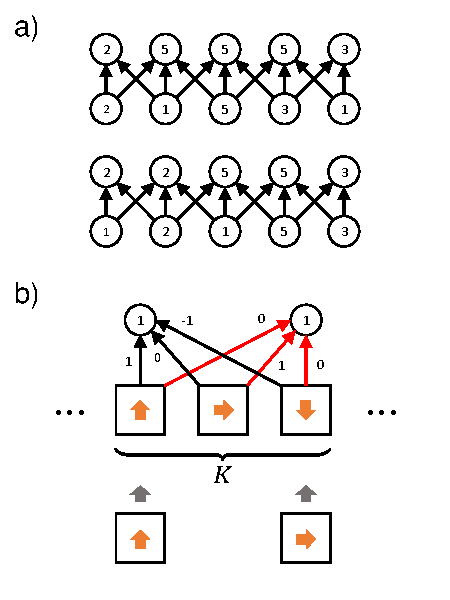
\includegraphics[width=3in]{figures/pooling.pdf}
    \caption{a) All the inputs of the pooling is shifted right by one. However, only one output value is changed. This shows that the output
            of the pooling is less sensitive to translation. 
            b) polling over the $K$ channel with rotated filters give results invariance to the rotations}
    \label{F:pooling}
\end{figure}

\subsection*{Invariance and equivariance of feature map}
\emph{Equivariance} refers to the property of mapping that perserve the transformation properties. 
For a network layer defined as a mapping $\Phi_l$ between input and output feature maps,  
Further denoting the action of the transformation $g$ on input and output feature maps by $T_{l-1}$ and $T_l$,
The condition that $\Phi_l$ is equivariant is:
\begin{equation}
    \Phi_l (T^{l-1}_g f_{l-1}) = T^l_g \Phi_l (f_{l-1}) \label{E:equivariant_condition}
\end{equation}

If $T^l_g$ is identity for all transformation $g$, We have the relationship:
\begin{equation}
    \Phi_l (T^{l-1}_g f_{l-1}) = \Phi_l (f_{l-1})\qquad \text{for all $g$} \label{E:invariant_condition}
\end{equation}
All transformation on the input feature map leave the output feature map invariant.

\subsection*{Equivariance of CNN on translation}
The effect of a translation $t = (u_t,v_t)$ on the feature map $f_{l-1}$ is given as:
\begin{equation}
    \label{E:translation_on_featuremap}
    (\Phi_t \circ f) (x) = f(x-t)
\end{equation}
This is show simply in Figure.\ref{F:3dnn_shift}
\begin{figure}[h]
    \centering
    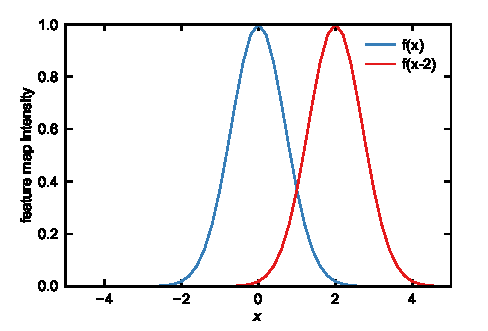
\includegraphics[width=3in]{figures/3dnn_shift.pdf}
    \caption{Apply a shift to resulting feature map is equivalent to a reverse shift in $x$. 
                In one-dimensional case with feature map given as $f\colon \mathbb{R} \to \mathbb{R}$,
                the feature map is translated to the right by $t = 2$, which correspond to the feature map $f(x-2)$}
    \label{F:3dnn_shift}
\end{figure}

We can show that convolution \eqref{E:convolution} is translation equivariant, satisfying Equation \eqref{E:equivariant_condition}
\begin{align*}
    (\Phi_l \circ \Phi_t \circ f_{l-1}) (x) &= \sum_y f_{l-1}(y-t) g_l(y-x) \\
    &= \sum_{y'} f_{l-1}(y') g_l(y'-x+t) \\
    &= \sum_{y'} f_{l-1}(y') g_l(y'-(x-t)) \\
    &= (\Phi_l \circ f_{l-1}) (x-t) \\ &= (\Phi_t \circ \Phi_l \circ f_{l-1}) (x)
\end{align*}
Therefore, $(\Phi_l \circ \Phi_t \circ f_{l-1}) (x) = (\Phi_t \circ \Phi_l \circ f_{l-1}) (x)$ and the convolution
is equivariant to translation. Similarly, both non-linear function and pooling are translation equivariant.

\vspace{10pt}
As shown in many studies, CNN predictions can be translation invariant: it can recognize the objects in 
image regardless of exact position of that object. However, we should distinguish the built-in equivariance 
from the learnt invariance\cite{kauderer-abrams_quantifying_2017}: 
by constructure, CNNs are equivariant to translation \footnote{as noted by E. K. Abrams, 2017, equivariance may be lost if pooling involve strides}, 
but it does not necessary lead to invariance in the prediction. 
CNN can be trained efficiently to identifying objects at different locations on the image with good performance.
The keypoint to achieve such invariance in the result seems to due to:
\begin{enumerate}
    \item Effect of pooling with decreasing spatial resolution with higher depth of features (channels) that contain highly extracted information.
    \item The larger field of reception at deeper layer, containing more spatial correlations. 
\end{enumerate}
%\begin{figure}[h!]
%    \centering
%    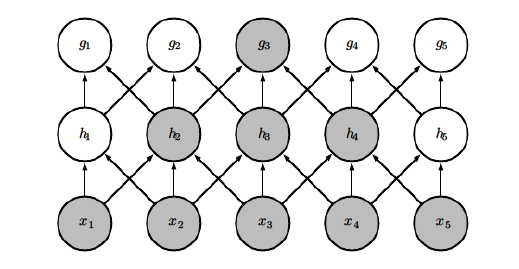
\includegraphics[width=3in]{figures/receptive_field_cnn.png}
%    \caption{The unit in deeper networks are indirectly connect to all or most of the image from the gradial convolution, even without pooling}
%    \label{F:larger_receptive_field}
%\end{figure}

\section{Group equivariant convolution networks}

Now, we generalize the standard CNN so that it is equivariant to general transformations. First, we will define transformation 
as elements in a group, then, we describe the group-equivariant version of CNN on discrete and continuous groups. 

\subsection*{Group of transformation}
Transformations of an object form a group $G$ since 
two successive transformations yield another transformation $g_1g_2\in G$ and 
we can always find a reverse transformation $g^{-1}g = e$, where $e$ is identity. We can now formally define the 
action of $g$ as linear transformation $T_g^l$ on vector space of feature maps at layer $l$. The linear transformation 
and the feature map space form a representation of the transformation group $G$. 
Now, we can define an equivariant CNN on group $G$ as follows: 
When the input on CNN is transformed as $f_0\to T_g^0f_0$ by $g\in G$, all features maps 
in the network: $f_l$ transform as $f_l \to T_g^lf_l$. 

We define the operation of $g$ on feature maps as: 
\begin{equation}
    \label{E:g_on_featuremap}
    (\Phi_g \circ f) (x) = f(g^{-1}x)
\end{equation}
This form is consistent with Equation \eqref{E:translation_on_featuremap}.
The standard CNN are equivariant to the group of translations, but not to rotations $r\in G$. This can be shown as follows:
\begin{align*}
    (\Phi_l \circ \Phi_r \circ f_{l-1}) (x) &= \sum_{y} f_{l-1}(y) g_l(ry-x) \\
    (\Phi_r \circ \Phi_l \circ f_{l-1}) (x) &= \sum_{y} f_{l-1}(y) g_l(y-r^{-1}x)
\end{align*}
This is shown in Figure \ref{F:rotation_is_not_equivariance}
\begin{figure}[h!]
    \centering
    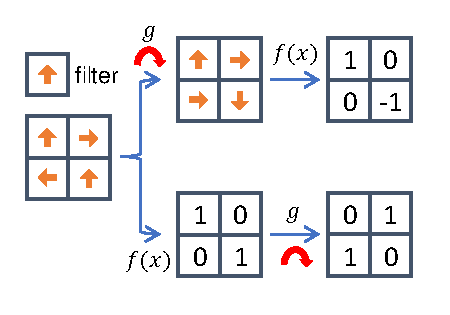
\includegraphics[width=3in]{figures/rotation_equivariance.pdf}
    \caption{
        Upper($[[L_r f]\star \psi] (x)$): we rotate the inputs, then perform correlation (rotating the feature map is equivalent to rotating the input with a reversed operation $g^{-1}$).
        Lower($[L_t[f\star \psi] ] (x)$): we first perform correlation, then rotate the resulting feature map }
    \label{F:rotation_is_not_equivariance}
\end{figure}

\subsection*{Homogeneous space and Quotient group}
We define a set $\calx$ to be the homogeneous space of a group $G$ if, taking any element $x_0\in \calx$,
all other elements in $\calx$ can be reached by applying $g\in G$ to $x_0$. 

Choosing $x_0$, All elements leave $x_0$ invariant $\{g\mid gx_0 = x_0\}$ is called a stabilizer of $x_0$ and is 
a normal subgroup of $G$. 
For normal subgroup $H$ of group $G$, $gH$ is called a left coset for a $g\in G$. 
The set of all left cosets $\{gH\mid g \in G\}$ form a quotient group, denoted as $G/H$.
The quotient group can be mapped to $\calx$ by a bijection: 
the group elements in the same coset are mapped to the same $x\in \calx$.

The key point here is to distinguish the group $G$ from its homogeneous space. It is more natural to define 
the convolution on homogeneous space of the transformation, than on transformation itself. This will be 
shown in the following.

\begin{comment}
\subsection*{General consideration}
In the standard convolution networks, each components are translational equivariant, meaning that the feature maps 
transform in the same way as the input image (Equation.\eqref{E:equivariant_condition}). Now, we extand 
convolution network to deal with general transformation, other than translation\cite{cohen_group_2016}.

We consider the group of transformation $G$ with group elements $g$ that can transform an image. 
We define an mages and stacks of feature maps as functions $f\colon \mathbb{Z}^2 \to \mathbb{R}^K$, which a a function
that map $(x,y)$ position of a figure to $K$ real numbers. For example, for an RGB color image. $K=3$ and 
we have three real value at a given pixel. 

As a concrete example for transformations, we consider that the input image are subject to transformation 
of operation in plane group $p4$, %for plane group, p is lower letter
which contain operation of 4-fold rotation around the origin and translations. 
we can parameterize any operation with integer number $r$, $u$ and $v$ as:
\begin{equation}
    g(r,u,v) = 
    \left[  
        \begin{matrix}
            \cos(r\pi / 2) & -\sin(r\pi / 2) & u \\
            \sin(r\pi / 2) & \cos(r\pi / 2) & v \\
            0 & 0 & 1
        \end{matrix}
    \right] \label{E:p4_g}
\end{equation}
where $r$ specifies four fold rotation and $t = (u,v)$ specifies translations. Operation of group element
on a vector $x = (i,j)$ is:
\begin{equation}
    gx = \left[  
        \begin{matrix}
            \cos(r\pi / 2) & -\sin(r\pi / 2) & u \\
            \sin(r\pi / 2) & \cos(r\pi / 2) & v \\
            0 & 0 & 1
        \end{matrix}
    \right] 
    \left[ \begin{matrix}i \\ j \\ 1 \end{matrix}\right]
\end{equation}
The transformations form a group, i.e.\,, successive combination of transformations in the group yield another transformation
belong to the same group. This can be directly verified by matrix multiplication with Equation.\eqref{E:p4_g}. 
We can say that the matrix of group operation and the corresponding vector space $(i,j)$ form a representation
of the group $p4$.

Formally, we define the transformation of feature maps as 
\begin{equation}
    [L_g f] (x) = f(g^{-1}x)
\end{equation}
Where $L_g$ denote transformation operation of the feature map corresponding to transformation $g$.
An illustration of the above definition is Figure.\,\ref{F:3dnn_shift}, which is a one-dimensional case with
feature map given as $f\colon \mathbb{Z} \to \mathbb{R}$. 
The feature map is translated to the right by $t = 2$, which correspond to the feature map $f(x-2)$


We use $l$ as index for layers in the network. 
In each layer, we take an input feature maps ($K^l$ channels) and correlate it with a 
set of $K^{l+1}$ filters. 
We define a filter function $\psi\colon \mathbb{Z}^2 \to \mathbb{R}^{K^l}$ (the dimensional of input and output of 
the filter is the same as that of the feature map). Filters act on feature map as:
\begin{align}
    [f * \psi] (x) &= \sum_y \sum_{k=1}^{K^l} f_k(y) \psi_k(x - y) && \text{convolution} \\
    [f \star \psi] (x) &= \sum_y \sum_{k=1}^{K^l} f_k(y) \psi_k(y - x) && \text{correlation} \label{E:correlation}
\end{align}
again, $x$ and $y$ are tuple denoting positions on the image. We consider the case of 
correlation in the following.

\begin{proposition}
    Correlation defined in Equation.\eqref{E:correlation} is equivariant with respect to translation.
\end{proposition}
\begin{proof}
    For a translation $t=(u,v)$, omitting the channel index $k$, we can show that
    \begin{align*}
        [[L_tf]\star \psi] (x)  &= \sum_y f(y-t) \psi(y-x) \\
                            &= \sum_y f(y) \psi(y-x+t) \\
                            &= \sum_y f(y) \psi(y-(x-t)) \\
                            &= [f\star \psi] (x-t) = [L_t[f\star \psi] ] (x) \qedhere
    \end{align*}
\end{proof}
where the symbol $[[L_tf]\star \psi](x)$ means we perform correlation on the transformed feature map $L_t f$ 
and $[L_t[f\star \psi] ] (x)$ means that we first perform correlation $[f\star \psi]$, 
than we perform a translation operation on the resulting feature map.
However, such correlation is not equivariant with respect to rotation $C_4$. This 
is shown in Figure.\ref{F:rotation_is_not_equivariance}, where the 
results of $[[L_r f]\star \psi] (x)$ and $[L_t[f\star \psi] ] (x)$ are different.

\end{comment}

\subsection*{$G$-convolution for discrete transformation}
We define convolution with respect to a group operation $g\in G$ ($G$-correlation) as:
\begin{equation}
    (\Phi_l \circ f_{l-1})(u) = \sum_{v\in G} f_{l-1}(v) g_l(u^{-1}v) \label{E:G-correlation}
\end{equation}
where $h \in G$.
We can see that the standard convolution Eq.\eqref{E:convolution} is a special case of the $g$-correlation.

Now, the feature map is defined on discrete 
trasnformation $f_l\colon G\to \mathbb{R}^{N_l}$, instead of $f\colon X\to \mathbb{R}^{N_l}$. 
Equation \eqref{E:G-correlation} is equivariant to transformation $g \in G$:
\begin{align*}
    (\Phi_l \circ \Phi_g \circ f_{l-1})(u) 
        &= \sum_{v\in G} f_{l-1}(g^{-1}v) g_l(u^{-1}v) \\
        &= \sum_{v'\in G} f_{l-1}(v') g_l(u^{-1}gv') \\
        &= \sum_{v'\in G} f_{l-1}(v') g_l((g^{-1}u)^{-1}v') \\
        &= \Phi_l \circ f_{l-1} (g^{-1}u) = (\Phi_g \circ \Phi_l \circ f_{l-1})(u)
\end{align*}

\subsection*{Nonlinearity}
We define a nonlinearity $\sigma\colon \mathbb{R} \to \mathbb{R}$ and write:
\begin{equation}
    (\Phi_{\sigma} \circ f) (u) = \sigma(f(u))
\end{equation}
i.e.\,,the nonlinearity is applied on the feature map. 
The combined operation satisfy Eq.\eqref{E:equivariant_condition}: 
\begin{align*}
    (\Phi_{\sigma} \circ \Phi_g \circ f)(u) &= \sigma(f(g^{-1}u)) \\
    &= (\Phi_g \circ \Phi_{\sigma} \circ f)(u)
\end{align*}
Therefore, nonlinear activation is equivariant 
and does not change the transformation properties of the feature map.

\subsection*{Pooling and subsampling}
Similar to standard , we define a pooling for feature map over $G$ as:
\begin{equation}
    (\Phi_p \circ f_{l-1})(u) = \max_{k \in uH} f(k)
\end{equation}
For $H \subset G$. Pooling is equivariant to $G$:
\begin{align*}
    (\Phi_p \circ \Phi_g \circ f_{l-1})(u) &= \max_{k \in uH} f_{l-1}(g^{-1}k) \\
        & = \max_{k'\in g^{-1}uH} f_{l-1}(k') \\
        &= (\Phi_p \circ f_{l-1})(g^{-1}u) = (\Phi_g \circ \Phi_p \circ f_{l-1})(u)
\end{align*}

Downsampling $f_{l}(u)$ require partitioning the group. As discussed previously, the natural way to partitioin a group
is by left cosets. We denote the left coset containing $u$ as $[uH]$, and the representive of $[uH]$ by $[u]$. The downsampled output feature map is 
$f_l\colon \mathcal{Y} \to \mathbb{R}^{N_l}$ where $\mathcal{Y}$ is the homogeneous space of $G/H$
Then, we can define downsampling with respect to $H$
\begin{equation}
    (\Phi_d \circ f_l)(y) = (\Phi_d \circ f_l(u)) = f_l([u])
\end{equation}
i.e., output feature map of the left coset containing $u$ has the same value for $u$ belong to the same left coset. 
This is equivariant to $G$:
\begin{align*}
    (\Phi_d \circ \Phi_g \circ f_l)(u) &= f_l(g^{-1}[u]) \\
    &= f_l([g^{-1}u]) \\
    &= (\Phi_d \circ f_l)(g^{-1}u) \\
    &= (\Phi_g \circ \Phi_d \circ f_l)(u)
\end{align*}
Furthermore, Downsampled feature map will be invariant to transformation $g$ 
if the coset contain $u$ is the same as the coset containing $g^{-1}u$.


%with the pooling domain a subgroup $U \subset G$. 
%The pooling domains $gU$ therefore partition 
%the group $G$ into left cosets. 
%It is shown that pooling commutes with group operation and therefore is equivariant.
%Pooling are reductions, therefore, the feature map after the 
%pooling over cosets will be defined on the quotient groups $G/U$. 

For example, for plane group $p4$, the group of all four rotations around a lattice points $R$ (point group) are a subgroup of $G$,
Taking $H = R$ for downsampling
the quotient group $p4/R$ is isomorphic to the translation of $p4$ and 
the rotation of the input feature map will have no effect on the output feature map (invariance is a special case of equivariance). 
%This is because a the coset is invariant 
%to its elements: $rR = R \ \text{for}\ r \in R$ and the feature map over $r$ is poolled over. This is similar to 
%the right panel in Figure.\ref{F:pooling}.

\section{Spherical convolution network}
Previous section extends the definition of convolution(correlation) to transformations operation of finite group. 
Now we consider extending it to continuous transformation\cite{cohen_spherical_2018} in three dimensional case. 

\subsection*{Correlation on sphere}
We consider an image on a unit sphere. We define the image on a sphere as function $f\colon S^2 \to \mathbb{R}^N$.
$S^2$ is the set of points $x\in \mathbb{R}^3$ on the unit sphere with position specified by $(\alpha, \beta)$ 
with $\alpha\in [0,2\pi]$ and $\beta \in [0,\pi]$. To specify a point at position $r$ within this unit sphere. 
We can give value $f(|r|)$ to the $\mathbf{x}$ on the sphere projected by that point. 

Contrary to the image defined on the sphere, rotation of the sphere is given by specified by three parameter: 
euler angles $\alpha$, $\beta$ and $\gamma$, $\gamma \in [0,2\pi]$. They correspond to rotation the north pool of the 
sphere to an specifid position $\alpha$, $\beta$, followed by a rotation around the axis. 
In cartesian coordinates, rotation can be specified as a $3\times 3$ matrix.

Using the notation developed above, we define rotated input image as: 
\begin{equation}
    (\Phi_r \circ f) (x) = f(r^{-1}x)
\end{equation}
For the first convolution, we have:
\begin{equation}
    \label{E:convolution_s2}
    (\Phi_l \circ f_{l-1}) (r) = \int_{s^2} f_{l-1}(x)g_l(r^{-1}x) dx
\end{equation}
with filter and input feature map defined on $S^2$. 
Since the following filter and feature map are defined on group $R$, We write convolution as:
\begin{equation}
    \label{E:convolution_r}
    (\Phi_l \circ f_{l-1}) (r) = \int_v f_{l-1}(v)g_l(r^{-1}v) du 
\end{equation}
$du$ is the integral element around the rotation $r$. In practice, the intergral over rotation can be transformed 
to be $\int\int\int d\alpha d\beta d\gamma$. There equation follows Equation \eqref{E:G-correlation} and therefore 
are equivariant to rotation.

Further simplification can be achieved utilizing the spherical harmonic decomposition. For 
a function on sphere, it can be decomposed using (real) spherical harmonics:
\begin{align}
    f(x) &= \sum_{0\leq l \leq b} \sum_{|m|\leq l} f_m^l Y_m^l(x) &  f_m^l &= \sum_{S^2} Y_m^l(x) f(x) dx  
    \label{E:s2_fft}
\end{align}
with $Y_m^l(x)$ the spherical harmonics and $b$ the bandwidth of the decomposition. 
Now, a feature map $f(x)$ is uniquely specified by its decomposition coefficient vector $\mathbf{f}_m^l$. 

Similarly, feature map defined on $R$ can be decomposed by Wigner D-function $D_{mn}^l(R)$,
with index range $-l \leq m,n \leq l$:
\begin{equation}
    f(r) = \sum_{0\leq l \leq b} (2l+1) \sum_{|m|,|n|\leq l} f_{mn}^l D_{mn}^l(r)
    \label{E:so3_fft}
\end{equation}.
$f(r)$ is equivalently specified by coefficients $\mathbf{f}_{mn}^l$.

R. Kondor and S. Trivedi showed the convolution theorem for convolution on groups, so that Equation \eqref{E:convolution_r} can be 
evaluated on the fourier space.


\begin{comment}
We define the transformation of the feature map as by rotation operator $L_R$. The transformed feature map is given 
by
\begin{equation}
    [L_R f](x) = f(R^{-1}x)
\end{equation}
Now, it is not possible to define convolution (correlation) as summations, as in Equation.\eqref{E:G-correlation}, 
because the group of rotation is continous. The natural extensio for continuous variable is given by inner product. 
For first layer that operate on the spherical image:
\begin{equation}
    [f \star \psi] (R) = \langle L_R \psi, f \rangle = \int_{S^2} \sum_{k=1}^{K^l} \psi_k(R^{-1}x) f_k(x) dx
\end{equation}

All later feature maps are function $f\colon SO(3)\to \mathbb{R}^K$. For $R, Q \in SO(3)$ we have:
\begin{equation}
    [L_R f](Q) = f(R^{-1}Q)
\end{equation}
and 
\begin{equation}
    [f \star \psi] (R) = \langle L_R \psi, f \rangle = \int_{SO(3)} \sum_{k=1}^{K^l} \psi_k(R^{-1}Q) f_k(Q) dQ
\end{equation}
where $\int_{SO(3)}$ can be expressed by $\int\int\int d\alpha d\beta d\gamma$. There equation follow 
Proposition.\ref{Prop:G-correlation} and therefore is equivariant with respect to transformations in the group.


\subsection*{Group equivariant CNN in Fourier transform}
For the calculation of convolution, it is convenient to use generalized fourier transformation. 
For any function on a sphere, we can define the fourier transformation and inverse transformation by:
\begin{align}
    f(x) &= \sum_{0\leq l \leq b} \sum_{|m|\leq l} f_m^l Y_m^l(x) &  f_m^l &= \sum_{S^2} \overline{Y_m^l(x)} f(x) dx  
\end{align}
with $Y_m^l(x)$ the spherical harmonics and $b$ the bandwidth of the decomposition. 
Similarly, any function on $R$ can be decomposed by Wigner D-function $D_{mn}^l(R)$,
with index range $-l \leq m,n \leq l$:
\begin{equation}
    f(R) = \sum_{0\leq l \leq b} (2l+1) \sum_{|m|,|n|\leq l} f_{mn}^l D_{mn}^l(R)
    \label{E:so3_fft}
\end{equation}.


Ignoring the summation over feature depth index $k$, to evaluate the correlation over rotation, we 
need to evaluate the integral:
\begin{align}
    &\int_{S^2} \psi(R^{-1}x) f(x) dx && \text{($S^2$-FT)}\\ 
    &\int_{SO(3)} \psi (R^{-1}Q) f (Q) dQ   && \text{($SO(3)$-FT)}
\end{align}
A practical method is to use the general fourier decomposition. Any function on a shpere $S^2$ can be decomposed using spherical
harmonics. 
\begin{align}
    f(x) &= \sum_{0\leq l \leq b} \sum_{|m|\leq l} f_m^l Y_m^l(x) &  f_m^l &= \sum_{S^2} \overline{Y_m^l(x)} f(x) dx  
    \label{E:s2_fft}
\end{align}
where $b$ is the bandwidth of the decomposition. Increasing $b$ increase the resolution of the function
\cite{esteves_learning_2018}.

Similarly, an function on $SO(3)$, $f\colon SO(3)\to \mathbb{R}$, can be decomposed into Wigner $D$-function $D_{mn}^l(R)$,
with index range $-l \leq m,n \leq l$:
\begin{equation}
    f(R) = \sum_{0\leq l \leq b} (2l+1) \sum_{|m|,|n|\leq l} f_{mn}^l D_{mn}^l(R)
    \label{E:so3_fft}
\end{equation}

With the definition Equation.\eqref{E:s2_fft} and \eqref{E:so3_fft}, The integrals are straight forward to compute, as shown 
in Appendix \ref{A:g-convolution}.

We can see that the result of the convolution can be expressed by the coefficients $\psi_{m}^l, f_{m}^l$
and $\psi_{mn}^l, f_{mn}^{l}$, which is passed down through the network, until an inverse transformation
are needed (for example, to pass through non-linear functions).

\subsection*{Clebsch-Gordan net}
R. Kondor et al. 2018 further generalize the spherical convolution network to be work completely on 
fourier space. In the spherical network as purposed previously, Nonlinearity require us to perform 
inverse fourier transform into the feature map on the group element space, therefore requires
multiple FT and IFT in a forward pass of the network. 

In R. Kondor et al. the nonlinearity is produced by tensor products, instead of $h\colon \mathbb{R}\to\mathbb{R}$.
By Clebsch-Gordan decomposition, the tensor product of two vector spaces is still a vector space of the representation
of the group. Using tensor product as non-linearity, therefore, all layers can operate on fourier components and 
the need for inverse fourier transformation is removed. 

\end{comment}

\section{Euclidean neural network}
\subsection*{Network on points}
Before going to rotational equivalent network on points, we first introduce two previous models that operates 
on points. Qi et al.\cite{qi_pointnet_2017} proposed a network (PointNet) design that operation on sets of points that respect 
the permutation invariance of the input points. The main structure of their network are can be summarized by 
the following operation:
\begin{equation}
    f({x_1,\dots,x_n}) \approx g(h(x_1),\dots,h(x_n)) \label{E:pointnet_operation}
\end{equation}
Here, function $f$ is a \emph{general} function $f\colon\, \text{set of points} \to \mathbb{R}$. This function 
is approximated using two function. $h\colon \mathbb{R}^N\to \mathbb{R}^K $ is a multi-layer neural network
and $g$ is some function that is symmetric to permutation, such as averaging or max-pooling. Note that the same 
$h$ is used for all points, so that the order of $x_i$ is the same of that of $h(x_i)$. 
In the first layer, $x_i$ denote inputs of coordination $(x,y,z)$, but they can be expanded to feature vector 
in higher dimensional feature space, associated on each point.
Two further features of their network are:
\begin{enumerate}
    \item Small modules are defined that take inputs of vector in feature space and output affine transformations that are used to 
            rotate all vectors. Therefore, this small modules are expected to learn the alignment of the points in the feature space 
            (3-D space or higher dimension feature space), which 
            are supposed to achieve invariant to geometric transformations.
    \item After some global feature are extracted using Equation \eqref{E:pointnet_operation}, they are concatenated to the individual
            feature vector on each point again. So that each points contains both local information and global information. The concatencated 
            feature can be passed throught MLPs to extract pointwise outputs
            \footnote{To give an example, if a set of point correspond to a table, then, the output global informations will be feature vector 
            is roughly correspond to a table, in global feature space. If we now concatenate this global information to individual point, we 
            can pass them to some further network, which will tell if some point belong to the legs of the table, or the surface.}. 
            This is similar to that used by [Chen et al. 2019].
\end{enumerate}

In their later work, called PointNet++\cite{qi_pointnet_2017-1}, points are further organized in a hierarchy so that some local feature are extracted from a subset of 
points. This is now every similar to pooling (loss of spatial resolution) in standard CNNs. 
Local features are again represented as points and organized again in the hierarchy. Therefore, such networks are stable against
some local deformations.

We also mention the Molecular deep tensor neural networks (MDTNN) by K. T. Sch\"{u}tt et al.\cite{schutt_quantum-chemical_2017} 
Their network operates on points but only 
using the relative distance as inputs. This choice apparently make the output invariant to geometric transformation of the input coordinates.

Their network start with a distance matrix $D$ with $d_{ij}$ giving the distance between atom $i$ and $j$, as well as a vector coefficients 
on atoms $\mathbf{c}_i \in \mathbb{R}^K$. 
In each layer, we update the coefficients:
\begin{equation}
    \mathbf{c}_i^{t+1} = \mathbf{c}_i^{t} + \sum_j v (\mathbf{c}, D) _{ij} \label{E:DTNN_refine}
\end{equation} 
$t$ refer to the layer index of the network,
matrix $V$ the interaction that is a function of $\mathbf{c}$ and $D$. The interaction $V$ as the shape $N\times N \times K$, where $N$ is
the number of atoms and $K$ is the depth of the features. Step of Equation \eqref{E:DTNN_refine} is also called a 'refinement'. 
We can also note that the summation over $j$ is similar to a pooling operation and the coefficients $c_i$ from later layers have a larger
field of reception (Figure.\ref{F:pooling}).
\begin{equation}
    v_{ij} = \tanh(c_j V D + W^c \mathbf{c}_j + W^d D + b_k )
\end{equation}
where all multiplication in this equation are matrix multiplication. 
$V\in \mathbb{R}^{K\times K \times N}$, $W^c\in \mathbb{R}^{K\times K}$ and $W^d\in \mathbb{R}^{K\times N}$ are the weights and 
$b_k$ are the weights.

After $T$ iteration, the network obtain coefficients $c_i$. At each point, the coefficients with length $K$ is then passed to 
a MLPs to extract physical quantities, such as atomic energies. However, we note that by construction, such network does not keep 
any information on the orientation, only distance information is used. The features on the point also does not have any rotational 
properties.

\subsection*{Euclidean neural network}

Euclidean nueral network purposed by Thomas et al. 2018\cite{thomas_tensor_2018} is different from the previous network in that
\emph{The euclidean neural network operate on points throughout the structure: convolution is performed on each point with respect to other points.}
Equivariance is achieved by their definition of point convoultion, but is simpler in the form because the discreteness of the 
points.

At each layer, each point $a$ in the point cloud are associated with a vector $(\mathbf{r}_a, \mathbf{x}_a)$ 
in the vector space $R^3 \oplus \mathcal{X}$, where $\oplus$ indicate direct sum. We require that vector space $\mathcal{X}$ are span 
by the spherical harmonics $Y_m^l$ for $0\leq l \leq b$ and $|m|\leq l$. We denote such a feature 
vector as $V_acm^l$, where $c$ denotes channels (depth). 
Under a rotation $R$ around a chosen origin, The input feature thus transforms as:
\begin{equation}
    (\mathbf{r}_{a}, V_{acm}^l) \to (R \mathbf{r}_{a}, \sum_{m'}D_{mm'}^l(R)V_{acm'}^l) \label{E:3dnn_rotation_input}
\end{equation}

We define a filter to be of the following form:
\begin{equation}
    F_{cm_f}^{l_f, l_i}(\mathbf{r}) =  R_c^{l_f, l_i} (r) Y_{m_f}^{l_f}(\mathbf{r})
\end{equation}
with $r = |\mathbf{r}|$, and $R_c^{l_f, l_i} (r)$ are the parameter of the filter function that can be learned.
The filter functions are equivariant to rotation:
\begin{align}
    F_{cm_f}^{l_f, l_i}(R\mathbf{r}) &= R_c^{l_f, l_i} (r) Y_{m_f}^{l_f}(R\mathbf{r}) \\
    &= R_c^{l_f, l_i} (r) \sum_{m_f'} D_{m_fm_f'}^{l_f}(R)  Y_{m_f}^{l_f}(\mathbf{r})
\end{align}
In the following, we will first define the components of the network.
Then we will show that they are equivariant to rotation. As well as 
invariant to translation and permutation.

\subsection*{Point convolution}
we define a convolution layer as:
\begin{align}
    V_{acm_o}^{l_o} &= L^{l_o}_{acm_o} (\mathbf{r}, V_{cm_i}^{l_i}) \notag\\
    &= \sum_{m_f, m_i} C^{l_o,m_o}_{(l_f, m_f)(l_i,m_i)} \sum_{b \in S} F_{cm_f}^{l_f, l_i}(\mathbf{r}_{ab}) V^{l_i}_{bcm_i} \label{E:3dnn_point_convolution}
\end{align}
where $l_i$ and $l_f$ is the rotation order of the input and the filter, $m = -l_f, \dots, l_f$ is the index of the basis function.
$C^{l_o,m_o}_{(l_f, m_f)(l_i,m_i)}$ is the \emph{Clebsch-Gordan coefficients}
Note that we do not contain index $a$ in \[L^{l_o}_{acm_o} (\mathbf{r}, V_{cm_i}^{l_i})\] because
the output depend on the feature vector $(\mathbf{r}, V_{cm_i}^{l_i})$ from all points in the set $S$.
Note that we can understand the 'convolution' as the convolution between the filter function and a delta function 
marking the position of the point, at $\mathbf{r}_{ab}$.

Since the output only depend on relative distance $\mathbf{r}_{ab} = \mathbf{r}_{a} - \mathbf{r}_{b} $, 
the output is invariant under a translation of all points. Also, the summation in Equation \eqref{E:3dnn_point_convolution}
means the result is invariant under permutation of points.

We can show that the above point convolution is equivariant to rotation (Appendix \ref{A:proof_equivariance_point}):
rotation on the input feature space $(l_i,m_i)$ 
correspond to rotation on output feature space $(l_o,m_o)$.

\subsection*{Self-interaction}
We define a self-interaction between the feature at each point $a$ as:
\begin{equation}
    V_{acm}^{l} = \sum_{c'} W^{l}_{cc'} V_{ac'm}^{l} 
\end{equation}
Such operation is independent on permutation and translation. It is also equivariant to rotation:
\begin{align*}
    [ W \circ R ] (V_{acm}^l) &= \sum_{c'} W^{l}_{cc'} \sum_{m'}D_{mm'}^l(R)V_{acm'}^l \\
                &= \sum_{m'}D_{mm'}^l(R) \sum_{c'} W^{l}_{cc'}  V_{acm'}^l \\
                &= [ R \circ W ] (V_{acm}^l)
\end{align*}
However, it should be noted that the self-interaction coefficients $W$ are used for every $m$. 
If for different $m$ we have different weight, we than have:
\begin{align*}
    [ W \circ R ] (V_{acm}^l) &= \sum_{c'} W^{lm}_{cc'} \sum_{m'}D_{mm'}^l(R)V_{acm'}^l \\
                &= \sum_{m'}D_{mm'}^l(R) \sum_{c'} W^{lm}_{cc'}  V_{acm'}^l 
\end{align*}
which is different from $\sum_{c'} W^{lm'}_{cc'}  V_{acm'}^l$ by first applying self-interaction.

\subsection*{Nonlinearity}
For nonlinearity, we can use:
\begin{align*}
    &h^l (V_{ac}^0 + b_c^0) & &\text{for $l=0$} \\ 
    &h^l (\|V\|_{ac}^l + b_c^l)V_{acm}^{l} &  &\text{for $l>0$} \label{E:3dnn_nonlinearity}
\end{align*}
with $h\colon \mathbb{R}\to \mathbb{R}$ and 
\[ \|V\|_{ac}^l = \sqrt{\sum_m |V_{acm}^l|^2} \]
Nonlinearity is invariant for permutation and translation. For rotation, 
because rotation does not change length in the vector space, $\|V\|_{ac}^l$ is 
therefore invariant of rotation:
\begin{equation}
    \|D(R)V\| = \|V\|
\end{equation}
Thus, $h^l (\|V\|_{ac}^l + b_c^l)$ is invariant with respect to rotation. 
The rotational properties is the output is solely given by $V_{acm}^{l}$.
Therefore, nonlinearity defined by Equation \eqref{E:3dnn_nonlinearity} is equivariant
with respect to rotation.

\subsection*{Relationship with spherical CNNs}
Here, we show the euclidean neural network can be understood as a special case of the more general spherical CNNs 
with fixed filter.
We first consider Equation \eqref{E:3dnn_point_convolution} with $l_i=m_i=0$, i.e., only scalars on each point. 
Omitting the channel index $c$, 
equation \eqref{E:3dnn_point_convolution} becomes:
\begin{align}
    V_{am}^{l} &= \sum_{b \in S} F_{m}^{l}(\mathbf{r}_{ab}) V_{b}  \notag\\
            &= \sum_{b \in S} \left[R^{l} (|r|)V_{b}\right] Y_{m}^{l}(\mathbf{x})
\end{align}
The part in square bracket is scalar value. This activation can be achieved by convoluting a filter with
\begin{equation}
    f(\mathbf{r}) = \sum_{b \in S} \left[R^{l} (|r|)V_{b}\right] \delta(\mathbf{x}_{ab})
\end{equation}
$\delta(\mathbf{x}_{ab})$ is zero unless the projection of the point b fall on the sphere at $\mathbf{x}_{ab}$. 
We define the filter as:
\begin{equation}
    g_l(x) = \sum_{0\leq l \leq b} \sum_{|m|\leq l} Y_m^l(x)
\end{equation}
Putting the above form into Equation \eqref{E:convolution_s2}:
\begin{align*}
    V_a (r) &= \int_{s^2} \sum_{b \in S} \left[R^{l} (|r|)V_{b}\right] \delta(\mathbf{x}_{ab}) \sum_{l,m} Y_m^l(r^{-1}x) dx \\
    &= \sum_{l,m} \sum_{b \in S} \left[R^{l} (|r|)V_{b}\right] Y_m^l(r^{-1}\mathbf{x}_{ab}) \\
    &= \sum_{l,m} \sum_{b \in S} \left[R^{l} (|r|)V_{b}\right] \sum_n D_{mn}^l(r^{-1}) Y_n^l(\mathbf{x}_{ab}) \\
    &= \sum_{l,m,n} D_{mn}^l(r^{-1}) \sum_{b \in S} \left[R^{l} (|r|)V_{b}\right] Y_n^l(\mathbf{x}_{ab})
\end{align*}
The coefficients \[V_{an}^l = \sum_{b \in S} \left[R^{l} (|r|)V_{b}\right] Y_n^l(\mathbf{x}_{ab})\] therefore uniquely define 
the feature map on $r$. It describes the local environment of the points equivariantly to rotation $r$.

If the point $b$ are associated with $l>0$, then we also need to take into account the rotational property of these points. This is 
achieved using the properties of Clebsch-Gordan coefficients, similar to the addition of angular moment in quantum mechanics.

\section{Applicaton}
In this section, we show that the rotational equivariant network is able to extract vector information 
on atoms, from the crystal structures.

\section{Conclusion}
We reviewed the basic ideal of translational and rotational equivariance that form the basis
for the development of rotational equivariant point convolution network. Furthermore, we showed
an application of the network. 

\printbibliography[title={Reference}]

\onecolumn

\appendices

\section{Equivariance of point convolution}
\label{A:proof_equivariance_point}
Here we show that the point convolution introduced as Equation \eqref{E:3dnn_point_convolution} is indeed 
rotational equivariant. Recall that the point convolution is given as:
\begin{align*}
    V_{acm_o}^{l_o} &= L^{l_o}_{acm_o} (\mathbf{r}, V_{cm_i}^{l_i}) \notag\\
    &= \sum_{m_f, m_i} C^{l_o,m_o}_{(l_f, m_f)(l_i,m_i)} \sum_{b \in S} F_{cm_f}^{l_f, l_i}(\mathbf{r}_{ab}) V^{l_i}_{bcm_i}
\end{align*}
Under transformation (Equation \eqref{E:3dnn_rotation_input}), we have:
\begin{align*}
    [ L \circ R ] (\mathbf{r}, V_{cm_i}^{l_i}) &= 
    L^{l_o}_{acm_o} (R \mathbf{r}, \sum_{m_i'}D_{m_im_i'}^{l_i}(R)V_{cm_i'}^{l_i}) \\
    &= \sum_{m_f, m_i} C^{l_o,m_o}_{(l_f, m_f)(l_i,m_i)} \sum_{b \in S} F_{cm_f}^{l_f, l_i}(R\mathbf{r}_{ab}) \sum_{m_i'}D_{m_im_i'}^{l_i}(R)V_{bcm_i'}^{l_i} \\
    &= \sum_{m_f, m_i} C^{l_o,m_o}_{(l_f, m_f)(l_i,m_i)} 
            \sum_{b \in S} R_c^{l_f, l_i} (r) \sum_{m_f'} D_{m_fm_f'}^{l_f}(R)  Y_{m_f}^{l_f}(\mathbf{r}_{ab}) \sum_{m_i'}D_{m_im_i'}^{l_i}(R)V_{bcm_i'}^{l_i} \\
    &= \sum_{m_o'} D_{m_om_o'}^{l_o}(R) \sum_{m_f, m_i} C^{l_o,m_o'}_{(l_f, m_f)(l_i,m_i)}  \sum_{b \in S} F_{cm_f}^{l_f, l_i}(\mathbf{r}_{ab}) V_{bcm_i}^{l_i} \\
    &= \sum_{m_o'} D_{m_om_o'}^{l_o}(R) L^{l_o}_{acm_o'} (\mathbf{r}, V_{cm_i}^{l_i}) = [ R \circ L ] (\mathbf{r}, V_{cm_i}^{l_i})
\end{align*}
which shows that point convolution is equivariant. We used the properties of Clebsch-Gordan coefficients:
\begin{equation}
    \sum_{m_fm_i} C^{l_o,m_o}_{(l_f, m_f)(l_i,m_i)} D_{m_fm_f'}^{l_f}(R) D_{m_im_i'}^{l_i}(R) = \sum_{m_o'} D_{m_om_o'}^{l_o}(R) C^{l_o,m_o'}_{(l_f, m_f')(l_i,m_i')}
\end{equation}


\end{document}